\documentclass[11pt]{article}

\usepackage[margin=1in]{geometry}
\usepackage[T1]{fontenc}
\usepackage{lmodern}
\usepackage{microtype}
\usepackage{amsmath,amssymb,amsthm,mathtools}
\usepackage{mathrsfs}
\usepackage[dvipsnames]{xcolor}
\usepackage[most]{tcolorbox}
\usepackage{tikz}
\usetikzlibrary{decorations.markings,patterns}
\usepackage{enumitem}
\usepackage{tocloft}
\usepackage[hidelinks]{hyperref}

\definecolor{courseblue}{HTML}{1F4E79}
\definecolor{lightblue}{HTML}{EAF2F8}
\definecolor{lightgreen}{HTML}{EAF7EA}
\definecolor{lightpink}{HTML}{FCE8EF}
\definecolor{lightyellow}{HTML}{FFF8D6}
\definecolor{warningyellow}{HTML}{D6A000}
\definecolor{exercisebg}{HTML}{FDEAEA}
\definecolor{exerciseframe}{HTML}{B54040}
\definecolor{examplebg}{HTML}{F4FAFE}
\definecolor{exampleframe}{HTML}{85C1E9}
\definecolor{darkgray}{HTML}{333333}
\definecolor{lightorange}{HTML}{FDEBD8}
\definecolor{orangeframe}{HTML}{E08A3C}
\definecolor{remarkbg}{HTML}{F3EEFB}
\definecolor{remarkframe}{HTML}{9B7FC9}

\setlength{\parindent}{0pt}
\setlength{\parskip}{0.45em}
\setlist[itemize]{topsep=0.25em,itemsep=0.15em}
\renewcommand{\cftsecleader}{\cftdotfill{\cftdotsep}}
\renewcommand{\cftsubsecleader}{\cftdotfill{\cftdotsep}}

\theoremstyle{plain}
\newtheorem{theorem}{Theorem}[section]
\newtheorem{proposition}[theorem]{Proposition}
\newtheorem{lemma}[theorem]{Lemma}
\newtheorem{corollary}[theorem]{Corollary}
\theoremstyle{definition}
\newtheorem{definition}[theorem]{Definition}
\newtheorem{example}[theorem]{Example}
\newtheorem{exercise}[theorem]{Exercise}
\newtheoremstyle{boldremark}
  {3pt}{3pt}{\normalfont}{}{\bfseries}{.}{.5em}
  {\thmname{#1}\thmnumber{ #2}\thmnote{ (#3)}}
\theoremstyle{boldremark}
\newtheorem*{remark}{Remark}
\theoremstyle{remark}
\newtheorem*{fact}{Fact}
\newtheorem*{warning}{Warning}

\tcolorboxenvironment{definition}{
  enhanced,
  unbreakable,
  colback=lightgreen,
  colframe=ForestGreen,
  boxrule=0.7pt,
  arc=2pt,
  left=6pt,
  right=6pt,
  top=5pt,
  bottom=5pt
}

\tcolorboxenvironment{remark}{
  enhanced,
  colback=remarkbg,
  colframe=remarkframe,
  before upper={\setlength{\parskip}{0.5em}},
  boxrule=0.7pt,
  arc=2pt,
  left=6pt,
  right=6pt,
  top=5pt,
  bottom=5pt
}

\tcolorboxenvironment{warning}{
  enhanced,
  colback=lightyellow,
  colframe=warningyellow,
  boxrule=0.7pt,
  arc=2pt,
  left=6pt,
  right=6pt,
  top=5pt,
  bottom=5pt
}

\tcolorboxenvironment{exercise}{
  enhanced,
  colback=exercisebg,
  colframe=exerciseframe,
  boxrule=1pt,
  arc=2pt,
  left=6pt,
  right=6pt,
  top=5pt,
  bottom=5pt
}

\tcolorboxenvironment{example}{
  enhanced,
  colback=examplebg,
  colframe=exampleframe,
  boxrule=0.7pt,
  arc=2pt,
  left=6pt,
  right=6pt,
  top=5pt,
  bottom=5pt
}

\numberwithin{equation}{section}

\newcommand{\be}{\begin{eqnarray}}
\newcommand{\ee}{\end{eqnarray}}
\newcommand{\C}{\mathbb{C}}
\newcommand{\R}{\mathbb{R}}
\newcommand{\N}{\mathbb{N}}
\newcommand{\Z}{\mathbb{Z}}
\DeclareMathOperator{\Log}{Log}
\DeclareMathOperator{\Arg}{Arg}

\DeclareMathOperator{\Hol}{\mathcal{H}\mathrm{ol}}
\DeclareMathOperator{\Real}{Re}
\DeclareMathOperator{\Imag}{Im}
\newcommand{\A}{\mathcal{A}}
\newcommand{\CT}{\C[[T]]}
\newcommand{\CLT}{\C((T))}
\tcbset{breakable}
% Compact spacing around diagrams; keep the main text at 11pt.
\newenvironment{lecturefigure}
 {\par\addvspace{0.25em}\begingroup\setlength{\parskip}{0pt}\centering}
 {\par\endgroup\addvspace{0.25em}}
\begin{document}

\begin{center}
  \colorbox{lightblue}{%
    \begin{minipage}{0.94\textwidth}
      \vspace{0.55em}
      \begin{tabular*}{\textwidth}{@{\extracolsep{\fill}}lr}
        {\color{courseblue}\bfseries\LARGE Lecture 21} &
        {\color{courseblue}\bfseries\LARGE MATH 411}\\[0.35em]
        \textbf{Fall 2026} & \textbf{Date: Oct 28, 2026}\\
        & \textbf{Instructor: Manish Patnaik}
      \end{tabular*}
      \vspace{0.45em}
    \end{minipage}}
\end{center}

\setcounter{tocdepth}{1}
\tableofcontents
\vspace{0.45em}

% Sources: handwritten Lecture 20, Oct. 28, pages 6--9. Order follows
% the handwritten notes: Morera's theorem, then Laurent series. The
% fundamental theorem of algebra (page 5) is covered in Lecture 20.
% Additional sources: handwritten Lecture 21, Oct. 31, pages 1--4,
% for annuli, Cauchy's formula, and examples. The Laurent expansion
% proof, uniqueness, and further examples continue in Lecture 22.
% The annulus case of Cauchy's formula is derived from the homotopy
% form (Lecture 18); the homology form is only remarked on.
In Lecture~20 we proved that every holomorphic function is analytic,
with the Cauchy estimates
\[
 |a_n|\leq\frac{\|f\|_{\gamma_R}}{R^n},\qquad
 a_n=\frac{f^{(n)}(z_0)}{n!}=\frac{1}{2\pi i}\int_{\gamma_R}
 \frac{f(\zeta)}{(\zeta-z_0)^{n+1}}\,d\zeta,
\]
whenever $\overline{D(z_0,R)}\subseteq U$, and we deduced Liouville's
theorem: \emph{every bounded entire function is constant}. We applied it
to prove the fundamental theorem of algebra. Today we prove Morera's
theorem and introduce Laurent series, which play the role of power
series on annuli. We state the Laurent expansion theorem and derive
Cauchy's formula on an annulus. The Laurent expansion proof, uniqueness,
and further examples are taken up in Lecture~22.

\section{Morera's theorem}
% Handwritten Lecture 20, page 6.
Morera's theorem is a converse to the Cauchy--Goursat theorem.

\begin{theorem}[Morera's theorem]\label{thm:morera}
Let $U\subseteq\C$ be open and $f$ continuous on $U$. Suppose
\[
 \int_{\partial Q}f=0
\]
for every closed rectangle $Q\subseteq U$ with sides parallel to the
axes. Then $f$ is holomorphic on $U$.
\end{theorem}

\begin{lecturefigure}
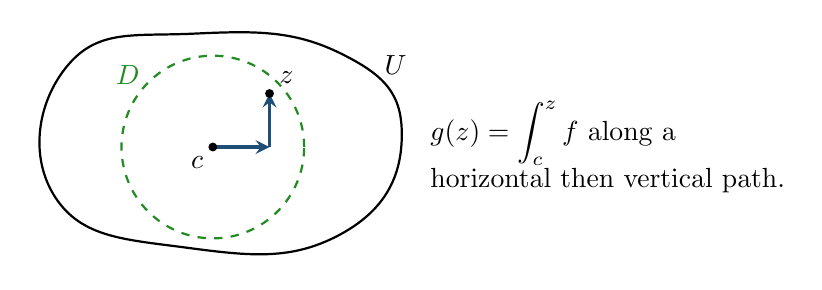
\begin{tikzpicture}[scale=0.8,>=stealth]
 \draw[thick] plot[smooth cycle,tension=0.8] coordinates
 {(-2.7,-0.8) (-2.5,1.3) (-0.5,1.8) (1.8,1.5) (2.8,0.2)
  (1.8,-1.4) (-0.6,-1.6)};
 \node at (2.7,1.3) {$U$};
 \draw[ForestGreen,thick,dashed] (-0.2,0) circle(1.45);
 \draw[courseblue,very thick,->] (-0.2,0)--(0.7,0);
 \draw[courseblue,very thick,->] (0.7,0)--(0.7,0.85);
 \fill (-0.2,0) circle(2pt) node[below left] {$c$};
 \fill (0.7,0.85) circle(2pt) node[above right] {$z$};
 \node[ForestGreen] at (-1.55,1.15) {$D$};
 \node[right,align=left] at (3.1,0)
 {$g(z)=\displaystyle\int_c^z f$ along a\\horizontal then vertical path.};
\end{tikzpicture}
\end{lecturefigure}

\begin{proof}
Holomorphy is a local property, so it suffices to work on a disc
$D\subseteq U$ with centre $c$. For $z\in D$ define
\[
 g(z)=\int_c^z f,
\]
integrating along the rectangular path that goes horizontally and then
vertically from $c$ to $z$; this path stays in $D$. This is exactly the
construction of a primitive on a disc that we used with the
Cauchy--Goursat theorem: there, the only input was that integrals of $f$
over boundaries of rectangles in $D$ vanish, which is now our hypothesis.
The same argument shows that $g$ is holomorphic on $D$ with $g'=f$.

By Theorem~1.1 of Lecture~20, $g$ is analytic on $D$, so its derivative
$g'=f$ is again holomorphic (Corollary~3.1 of Lecture~20). Thus $f$
is holomorphic on $D$, and hence on $U$.
\end{proof}

\begin{exercise}
Let $f_n$ be holomorphic on an open set $U$ and suppose $f_n\to f$
uniformly on every closed disc contained in $U$. Use
Proposition~2.1 of Lecture~20, the Cauchy--Goursat theorem, and
Morera's theorem to show that $f$ is holomorphic on $U$.
\end{exercise}

\section{Laurent series}
% Handwritten Lecture 20, pages 7--9.
Power series model holomorphic functions on discs. To model functions on
annuli, such as $1/z$ or $e^{1/z}$ near $0$, we allow negative powers.
In Lecture~6 we met the formal Laurent series $\CLT$, which have only
finitely many negative powers. We now allow infinitely many terms in both
directions.

\begin{definition}
A \emph{Laurent series} (centred at $0$) is an expression
\[
 f(z)=\sum_{n=-\infty}^{\infty}a_nz^n .
\]
We split it into
\[
 f_+(z)=\sum_{n\geq0}a_nz^n,\qquad f_-(z)=\sum_{n<0}a_nz^n
 =\sum_{m\geq1}a_{-m}\Bigl(\frac1z\Bigr)^m,
\]
and say that the Laurent series \emph{converges} at $z$ if both $f_+(z)$
and $f_-(z)$ converge.
\end{definition}

To understand $f_-$, consider the ordinary power series in a new
variable $T$:
\[
 a_{-1}T+a_{-2}T^2+a_{-3}T^3+\cdots .
\]
Suppose it has radius of convergence $\rho_->0$, so it converges for
$|T|<\rho_-$. Substituting $T=1/z$, the series $f_-(z)$ converges for
\[
 \frac{1}{|z|}<\rho_-,\qquad\text{i.e.}\qquad |z|>r:=\frac{1}{\rho_-}.
\]
If $f_+$ has radius of convergence $R$, then $f_+$ converges for
$|z|<R$, and $f_-$ converges for $|z|>r$. When $r<R$, both converge on
the open annulus $r<|z|<R$.

\begin{lecturefigure}
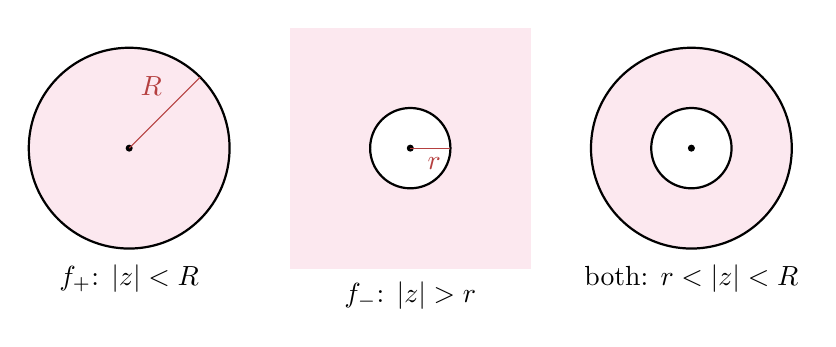
\begin{tikzpicture}[scale=0.85]
 \begin{scope}
  \fill[lightpink] (0,0) circle(1.5);
  \draw[thick] (0,0) circle(1.5);
  \fill (0,0) circle(1.5pt);
  \draw[exerciseframe] (0,0)--(1.06,1.06) node[pos=0.6,above left]{$R$};
  \node[below] at (0,-1.6) {$f_+$: $|z|<R$};
 \end{scope}
 \begin{scope}[xshift=4.2cm]
  \fill[lightpink] (-1.8,-1.8) rectangle (1.8,1.8);
  \fill[white] (0,0) circle(0.6);
  \draw[thick] (0,0) circle(0.6);
  \fill (0,0) circle(1.5pt);
  \draw[exerciseframe] (0,0)--(0.6,0) node[pos=0.6,below]{$r$};
  \node[below] at (0,-1.85) {$f_-$: $|z|>r$};
 \end{scope}
 \begin{scope}[xshift=8.4cm]
  \fill[lightpink] (0,0) circle(1.5);
  \fill[white] (0,0) circle(0.6);
  \draw[thick] (0,0) circle(1.5);
  \draw[thick] (0,0) circle(0.6);
  \fill (0,0) circle(1.5pt);
  \node[below] at (0,-1.6) {both: $r<|z|<R$};
 \end{scope}
\end{tikzpicture}
\end{lecturefigure}

For $0\leq r<R\leq\infty$ write
\[
 A(r,R)=\{z\in\C:\ r<|z|<R\}
\]
for the \emph{open} annulus. We allow $r=0$ (a punctured disc, or
$\C\setminus\{0\}$ if also $R=\infty$) and $R=\infty$ (the exterior of a
disc).

% Handwritten Lecture 21, page 1.
In the splitting above, $f_+$ is a power series in $z$ and $f_-$ is a power series in $1/z$
without constant term. On a closed disc strictly inside its disc of
convergence a power series converges uniformly, so a Laurent series that
converges on $A(r,R)$ converges uniformly on every closed annulus
$\{s\leq|z|\leq S\}$ with $r<s<S<R$.

For $\rho>0$, let $C_\rho(t)=\rho e^{it}$, $0\leq t\leq2\pi$, be the
positively oriented circle of radius $\rho$ centred at $0$.

\begin{lecturefigure}
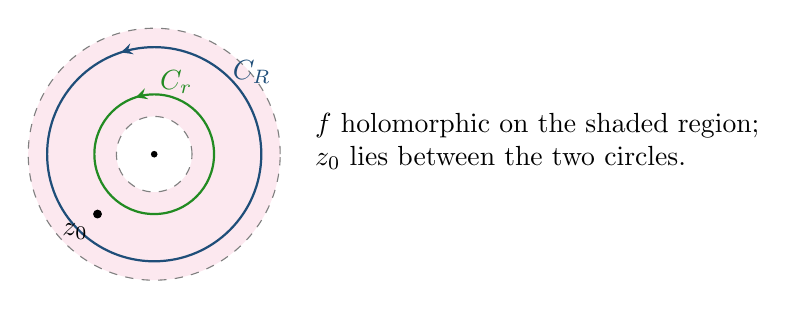
\begin{tikzpicture}[scale=0.8,>=stealth]
 \fill[lightpink] (0,0) circle(2);
 \fill[white] (0,0) circle(0.6);
 \draw[gray,dashed] (0,0) circle(2);
 \draw[gray,dashed] (0,0) circle(0.6);
 \draw[courseblue,thick,postaction={decorate},decoration={markings,
  mark=at position 0.3 with {\arrow{>}}}] (1.7,0) arc(0:360:1.7);
 \draw[ForestGreen,thick,postaction={decorate},decoration={markings,
  mark=at position 0.3 with {\arrow{>}}}] (0.95,0) arc(0:360:0.95);
 \fill (0,0) circle(1.5pt);
 \node[courseblue] at (1.55,1.3) {$C_R$};
 \node[ForestGreen] at (0.35,1.15) {$C_r$};
 \fill (-0.9,-0.95) circle(2pt) node[below left]{$z_0$};
 \node[right,align=left] at (2.4,0.2)
 {$f$ holomorphic on the shaded region;\\
  $z_0$ lies between the two circles.};
\end{tikzpicture}
\end{lecturefigure}

For $0<r<R<\infty$, the closure of $A(r,R)$ is the closed annulus
\[
 \overline{A(r,R)}=\{z\in\C:\ r\leq|z|\leq R\}.
\]
Lang, Chapter~V, \S2, Theorem~2.1, uses this closed annulus and assumes
that $f$ is holomorphic on an open set containing it; we use the same
hypothesis in the theorem below. Just as power series model holomorphic functions
on discs, Laurent series model holomorphic functions on annuli.

\begin{theorem}[Laurent expansion]\label{thm:laurent}
Let $0<r<R<\infty$ and let $f$ be holomorphic on $\overline{A(r,R)}$
(that is, on an open set containing $\overline{A(r,R)}$).
Let $C_R$ and $C_r$ be the positively oriented
circles $|\zeta|=R$ and $|\zeta|=r$, and set
\[
 a_n=\frac{1}{2\pi i}\int_{C_R}\frac{f(\zeta)}{\zeta^{n+1}}\,d\zeta
 \quad(n\geq0),\qquad
 a_n=\frac{1}{2\pi i}\int_{C_r}\frac{f(\zeta)}{\zeta^{n+1}}\,d\zeta
 \quad(n<0).
\]
Then for $r<|z|<R$,
\[
 f(z)=\underbrace{\sum_{n\geq0}a_nz^n}_{f_+(z)}
 +\underbrace{\sum_{n<0}a_n\Bigl(\frac1z\Bigr)^{-n}}_{f_-(z)},
\]
and the convergence is uniform on every smaller closed annulus
$s\leq|z|\leq S$ with $r<s<S<R$.
\end{theorem}
% Handwritten page 9 writes f(\zeta)/\zeta^n for n<0 and omits 1/(2\pi i);
% corrected so that both coefficient formulas have the same form.

\begin{lecturefigure}
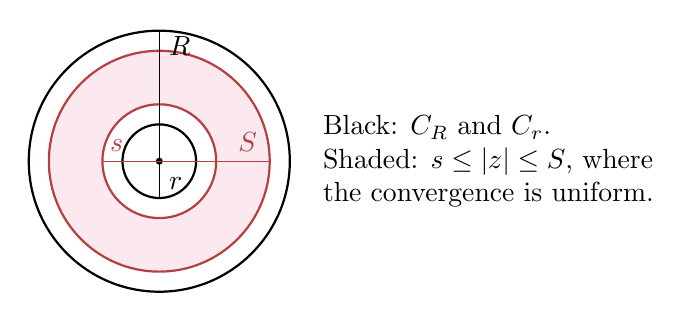
\begin{tikzpicture}[scale=0.85]
 \fill[lightpink] (0,0) circle(1.65);
 \fill[white] (0,0) circle(0.85);
 \draw[thick] (0,0) circle(1.95);
 \draw[thick] (0,0) circle(0.55);
 \draw[exerciseframe,thick] (0,0) circle(1.65);
 \draw[exerciseframe,thick] (0,0) circle(0.85);
 \fill (0,0) circle(1.5pt);
 \draw (0,0)--(0,1.95) node[pos=0.88,right]{$R$};
 \draw (0,0)--(0,-0.55) node[pos=0.6,right]{$r$};
 \draw[exerciseframe] (0,0)--(-0.85,0) node[pos=0.75,above]{$s$};
 \draw[exerciseframe] (0,0)--(1.65,0) node[pos=0.8,above]{$S$};
 \node[right,align=left] at (2.3,0)
 {Black: $C_R$ and $C_r$.\\
  Shaded: $s\leq|z|\leq S$, where\\
  the convergence is uniform.};
\end{tikzpicture}
\end{lecturefigure}

The proof, which again starts from Cauchy's formula and two geometric
series, is given in Lecture~22.

Recall that ``$f$ is holomorphic on
$\overline{A(r,R)}$'' means holomorphic on an open set containing the
closed annulus, including both boundary circles.

\begin{remark}[The case of a disc]
	% Handwritten Lecture 21, top of page 2.
	If $f$ is holomorphic on the whole closed disc $|z|\leq R$ (no hole),
	then for $n<0$ the function $\zeta^{-n-1}f(\zeta)$ is holomorphic on that
	disc, so $a_n=0$ by Cauchy's theorem. Then $f=f_+$, and we are back to the
	usual statement of Lecture~20:
	\[
	f(z)=\sum_{n\geq0}a_nz^n,\qquad
	a_n=\frac{1}{2\pi i}\int_{C_R}\frac{f(\zeta)}{\zeta^{n+1}}\,d\zeta .
	\]
\end{remark}



\begin{example}[The annulus matters]\label{ex:annulus-matters}
The function $f(z)=1/(z-1)$ is holomorphic on $\C\setminus\{1\}$.
On the disc $|z|<1$,
\[
 \frac{1}{z-1}=-\frac{1}{1-z}=-\sum_{n\geq0}z^n,
\]
so $f=f_+$ and $f_-=0$. On the region $|z|>1$, instead,
\[
 \frac{1}{z-1}=\frac1z\,\frac{1}{1-1/z}=\sum_{m\geq1}\Bigl(\frac1z\Bigr)^m,
\]
so $f=f_-$ and $f_+=0$. The same function has different Laurent
expansions on different annuli.
\end{example}

\begin{exercise}
Find the Laurent expansion of $e^{1/z}$ on $0<|z|<\infty$. Which
coefficients $a_n$ are nonzero? Compare with the coefficient formula of
Theorem~\ref{thm:laurent} for $n=-1$.
\end{exercise}


\subsection{Cauchy's formula on an annulus}
% Handwritten Lecture 21, page 2.
The key input is a version of Cauchy's formula in which the contour is the
boundary of the annulus: the outer circle counterclockwise and the inner
circle clockwise. Recall from Lecture 18.

\begin{lemma}[Concentric circles]\label{lem:concentric}
Let $0<\rho_1<\rho_2$ and let $h$ be holomorphic on an open set containing
$\{\rho_1\leq|z|\leq\rho_2\}$. Then
\[
 \int_{C_{\rho_1}}h(\zeta)\,d\zeta=\int_{C_{\rho_2}}h(\zeta)\,d\zeta.
\]
\end{lemma}


\begin{proposition}[Cauchy's formula on an annulus]\label{prop:annulus-cauchy}
Let $f$ be holomorphic on $\overline{A(r,R)}$, where $0<r<R<\infty$. Then for
every $z_0$ with $r<|z_0|<R$,
\[
 \boxed{\displaystyle
 f(z_0)=\frac{1}{2\pi i}\int_{C_R}\frac{f(\zeta)}{\zeta-z_0}\,d\zeta
 -\frac{1}{2\pi i}\int_{C_r}\frac{f(\zeta)}{\zeta-z_0}\,d\zeta.}
\]
\end{proposition}
\begin{proof}
Define
\[
 g(\zeta)=\frac{f(\zeta)-f(z_0)}{\zeta-z_0}\quad(\zeta\ne z_0),
 \qquad g(z_0)=f'(z_0).
\]
Away from $z_0$, $g$ is clearly holomorphic. Since $f$ is holomorphic near
$z_0$, Lecture~20 gives a convergent power series
\[
 f(\zeta)=\sum_{k\geq0}b_k(\zeta-z_0)^k
 \qquad(|\zeta-z_0|<\delta)
\]
for some $\delta>0$, with $b_0=f(z_0)$ and $b_1=f'(z_0)$. For
$0<|\zeta-z_0|<\delta$, subtracting $b_0$ and dividing by $\zeta-z_0$ gives
\[
 g(\zeta)=\frac{f(\zeta)-f(z_0)}{\zeta-z_0}
 =\sum_{k\geq1}b_k(\zeta-z_0)^{k-1}.
\]
The shifted power series converges throughout $|\zeta-z_0|<\delta$.
At $\zeta=z_0$ its value is $b_1=f'(z_0)=g(z_0)$, so it represents $g$
on the whole disc, including its centre. Hence $g$ is holomorphic at
$z_0$. Thus $g$ is holomorphic on a neighbourhood of the closed
annulus, and Lemma~\ref{lem:concentric} gives
$\int_{C_R}g=\int_{C_r}g$, that is,
\[
 \int_{C_R}\frac{f(\zeta)}{\zeta-z_0}\,d\zeta
 -f(z_0)\int_{C_R}\frac{d\zeta}{\zeta-z_0}
 =\int_{C_r}\frac{f(\zeta)}{\zeta-z_0}\,d\zeta
 -f(z_0)\int_{C_r}\frac{d\zeta}{\zeta-z_0}.
\]
Since $|z_0|<R$, the local Cauchy formula (Lecture~18) applied to the
constant function $1$ gives $\int_{C_R}d\zeta/(\zeta-z_0)=2\pi i$. Since
$|z_0|>r$, the function $1/(\zeta-z_0)$ is holomorphic on the disc
$|\zeta|<|z_0|$, which contains $C_r$, so $\int_{C_r}d\zeta/(\zeta-z_0)=0$
by Cauchy's theorem on a disc. Rearranging gives the formula.
\end{proof}

\begin{remark}[The homology form of Cauchy's theorem]
Actually there is a more general fact: if $\gamma$ is a
(formal sum of) closed curves in $U$ that does not wind around any point
outside $U$, then
\[
 \frac{1}{2\pi i}\int_\gamma\frac{f(\zeta)}{\zeta-z_0}\,d\zeta
 =n(\gamma,z_0)\,f(z_0),\qquad
 n(\gamma,z_0)=\frac{1}{2\pi i}\int_\gamma\frac{d\zeta}{\zeta-z_0},
\]
where $n(\gamma,z_0)$ is the \emph{winding number} of $\gamma$ around $z_0$.
For $\gamma=C_R-C_r$ and $z_0$ in the annulus, $n(\gamma,z_0)=1-0=1$, which
is Proposition~\ref{prop:annulus-cauchy}. We will not need the general
statement.
\end{remark}

\begin{lecturefigure}
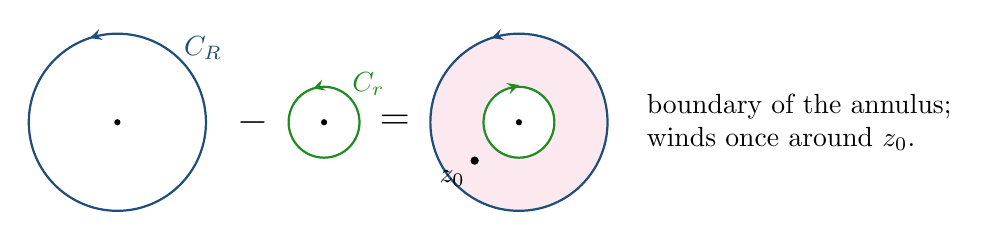
\begin{tikzpicture}[scale=0.75,>=stealth]
 \begin{scope}
  \draw[courseblue,thick,postaction={decorate},decoration={markings,
   mark=at position 0.3 with {\arrow{>}}}] (1.5,0) arc(0:360:1.5);
  \node[courseblue] at (1.45,1.25){$C_R$};
  \fill (0,0) circle(1.5pt);
 \end{scope}
 \node at (2.3,0) {\Large$-$};
 \begin{scope}[xshift=3.5cm]
  \draw[ForestGreen,thick,postaction={decorate},decoration={markings,
   mark=at position 0.3 with {\arrow{>}}}] (0.6,0) arc(0:360:0.6);
  \node[ForestGreen] at (0.75,0.65){$C_r$};
  \fill (0,0) circle(1.5pt);
 \end{scope}
 \node at (4.7,0) {\Large$=$};
 \begin{scope}[xshift=6.8cm]
  \fill[lightpink] (0,0) circle(1.5);
  \fill[white] (0,0) circle(0.6);
  \draw[courseblue,thick,postaction={decorate},decoration={markings,
   mark=at position 0.3 with {\arrow{>}}}] (1.5,0) arc(0:360:1.5);
  \draw[ForestGreen,thick,postaction={decorate},decoration={markings,
   mark=at position 0.3 with {\arrow{<}}}] (0.6,0) arc(0:360:0.6);
  \fill (0,0) circle(1.5pt);
  \fill (-0.75,-0.65) circle(2pt) node[below left]{$z_0$};
 \end{scope}
 \node[right,align=left] at (8.8,0)
 {boundary of the annulus;\\ winds once around $z_0$.};
\end{tikzpicture}
\end{lecturefigure}

\end{document}
